
\section{学生処分問題と熊野寮自治会の対応}
\label{sec:shobun}
\bunsekisha{文責}{対処分戦略推進局}


高校でも生徒が「問題」行動を起こした時に、反省文を書かされたり、停学にさせられるなどの処分が行われることがありますが、京大でも似たような措置が不当かつ恣意的に行われ、学生の自由と人権が抑圧されているという現状があります。近年の京大では吉田寮問題や立て看問題(後述)など、大学当局からの学生への抑圧が強まっており、徐々に自由な雰囲気を失いつつあります。しかし京大には、今の自由を守ろう、いや、今よりもっと自由な京大を作ろう、と考え行動している学生がまだまだたくさんいます。処分はそうした「問題」行動を起こす学生への脅しとして使われてしまっているのです。ここでは、熊野寮の要求書提出時に職員に抗議した3名の寮生が無期停学処分にされたことと、京大の二次試験の会場に像を設置した寮生1名が\ruby{譴責}{けん|せき}処分にされたことの3つの事例を紹介し、何が問題なのか、今まで寮としてどんな対応をしてきたか、これからどうするべきか、ということについて書きたいと思います。

\begin{shadebox}
{\large\textbf{出る順! 処分問題単語帳}}
\begin{description}
    \item[処分(正式には「学生懲戒処分」)] 当局が「問題だ」と考える学生に当局が与える罰。京都大学学生懲戒規定(\url{https://www.kyoto-u.ac.jp/uni_int/kitei/reiki_honbun/w002RG00000283.html})に手続きの定めがある。要は、当局の都合の悪い学生を屈服されるための最終手段。 処分の軽重は学部の教授会が上申するが、最終的には当局が決定する。
    \item[当局(「大学当局」「京大当局」とも)] 法律上京都大学で一番偉い「役員会」(「理事会」と言われることも多い)を中心とした大学執行部やその意向を受けて学生と対峙することになる職員全般を指す。単に「京大」とか「京都大学」だと、教授会のことを指すのか、役員会のことを指すのか、僕ら学生のことを指すのか、それともそうしたものを全部ひっくるめているのか、分からないので「当局」は便利な言葉だ。処分問題に限らず京大内では頻出語なので絶対に憶えておこう。
    \item[教授会] 	各学部(学科)の教員で構成される会議体で、昔はとっても偉くて学部ごとの独立が強かった(学部自治)けど、今は役員会の方が偉くなってしまった。
    \item[学生自治会] 学部や寮などに組織されている学生全員加盟制の自治会。学生のために自分たちで動いたり、当局と交渉したりしている。学生自治会がない学部や寮もある。熊野寮自治会は学生自治会の一つだ。
    \item[停学] 大学構内に入れず、当然授業も受けれず、図書館も使えないのに授業料は満額取られてしまうというヒドい処分。有期停学(6月未満)と無期停学がある。無期停学よりヒドい処分としては、京大に在籍したという記録自体が抹消され、学生の身分も剥奪される「放学処分」がある。
    \item[\ruby{譴責}{けん|せき}] 学部長に怒られるという処分。停学よりは軽いが、実質的には「次やれば停学」を言い渡されるようなもので学生の威圧には十分だ。
\end{description}
\end{shadebox}


\subsection{寮生に暴行を振るう職員に抗議しただけで無期停学!?}
熊野寮自治会は自治会として大学当局に要求することを要求書にまとめて、当局の「厚生課」と呼ばれる窓口に提出することあります。事件が起こったのは2018年10月の要求書提出のときです。一人の寮生(以下Aとします)が職員に取り囲まれ、暴行を受けました。Aさんが覆面をしていたため、当局はこの行為を「不審者対応」であると称しています。これに対して、提出に参加していた3名の寮生が、職員とAさんの間に割って入り、職員に抗議しました。この抗議が「業務の妨害」とみなされ、2019年9月に3名に対して無期停学処分が下されました。このうち1名はいまだに停学が続いています。


\newpage

\subsection{オルガ像を設置して譴責処分!?}

\begin{wrapfigure}{r}{8zw}
    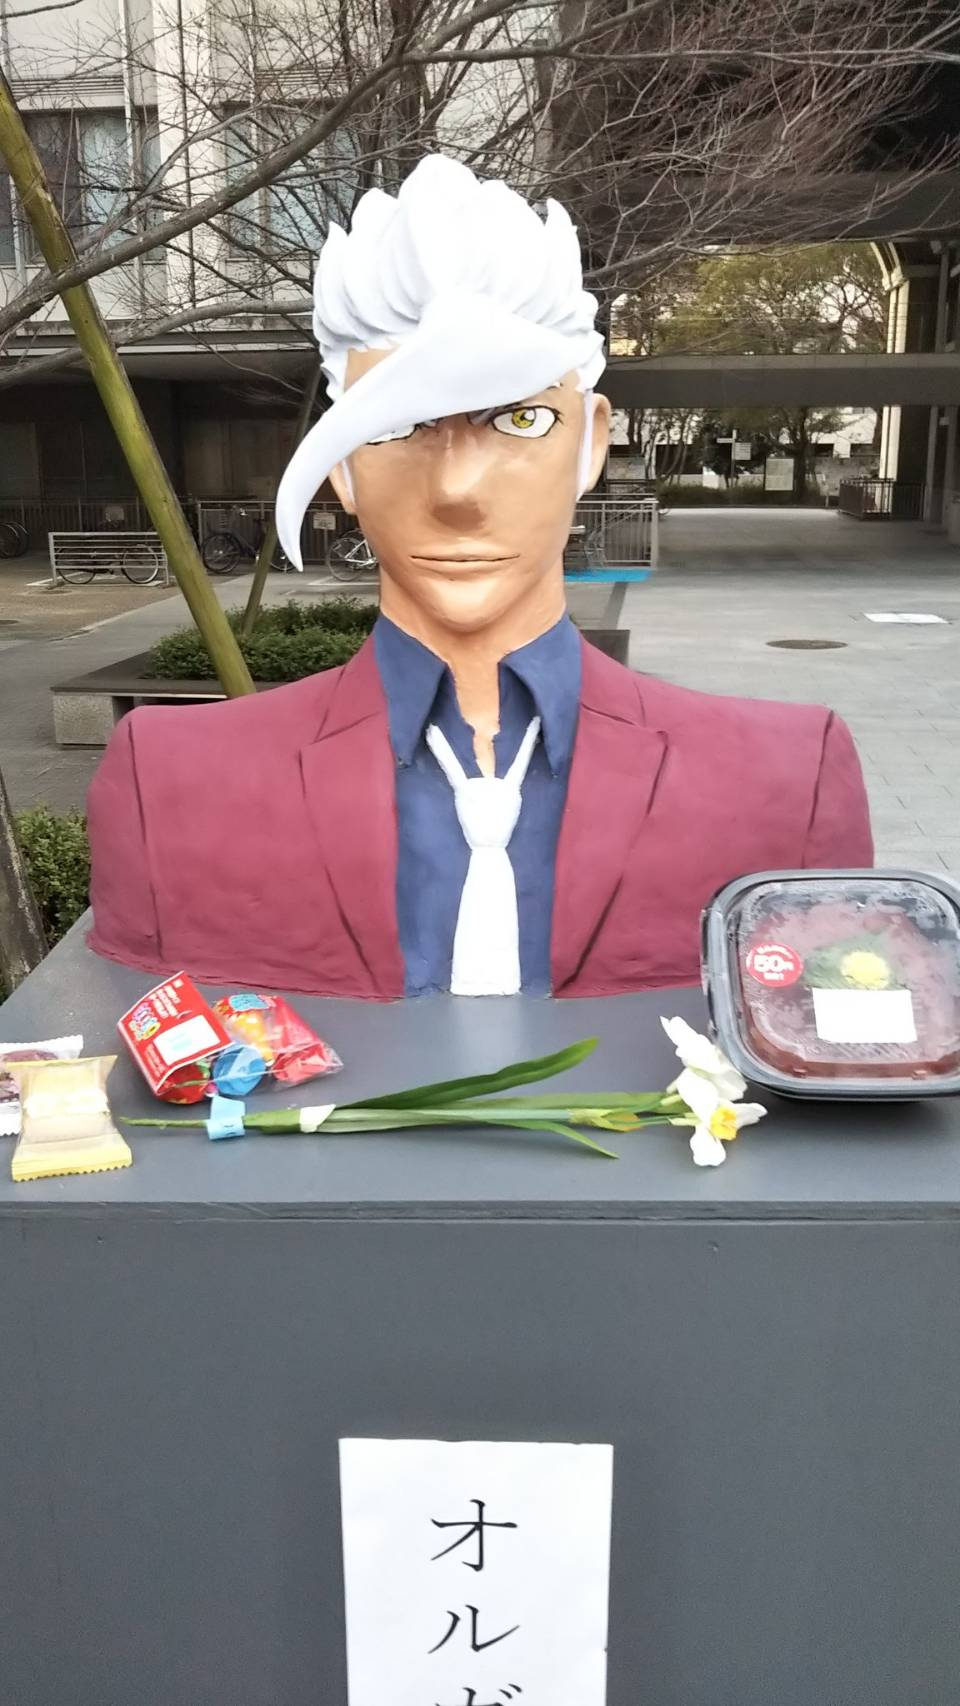
\includegraphics[width=8zw]{gazo/oruga.jpg}
    \captionsetup{labelformat=empty,labelsep=none}
    \caption{オルガ像}
\end{wrapfigure}

読んでいる人の多くが京大の二次試験でパンフを受け取ったと思います。今年はコロナ対策でどうなっているか分かりませんが、京大の二次試験は様々な学生が立て看や像を立てたり、入寮パンフを配ったり、受験生と麻雀をしたりと、構内は受験生激励で非常ににぎやかになります(もちろん試験時間中は静かです)。2019年の入試会場での『機動戦士ガンダム 鉄血のオルフェンズ』のキャラクター「オルガ・イツカ」の像設置も、こうした激励行為の一環として行われました。しかし、この行為が「迷惑行為」「業務の妨害」とみなされ、2020年1月にオルガ像を設置した寮生1名に対して、譴責処分が下りました。

\subsection{時計台に登ろうとして処分!?}
熊野寮祭の恒例企画と言えば「時計台占拠」。京大の時計台に\ruby{梯子}{はし|ご}を掛けて登る企画です。10年以上続いてきた企画で、昔は職員も「危ないからやめなさい」と言いつつ、梯子を支えたり、写真撮影を手伝ったりと安全な企画の貫徹に気を配っていました。しかし、ここ数年は一転し、大勢の職員が梯子を奪ってきたり、掛けられた梯子を揺らしたり、警察を構内に導入して妨害するなど、強固な弾圧に及んでいます。こうした中、2020年に行われた時計台占拠に参加したとして9名の学生に処分に向けた呼び出しがあり、最終的に2021年11月に卒業した1名を除く8名に対し、有期停学や譴責といった処分が下りました。


\subsection{何が問題なの?}
2つの処分の経緯を軽く見ましたが、「処分されて当たり前やん」と思ったかもしれません。しかし、この処分は不当なものです。問題は
\begin{enumerate}
    \item 処分は被処分者の人権を侵害するものである
    \item 被処分者の行為は問題のあるものではない(なのに恣意的に処分規定が適用されている)
    \item 逆に職員の行為こそ問題のあるものだ(なのにそれについては検証されていない)
    \item 処分は学生を威圧し、学生の自由を弾圧するために用いられている
\end{enumerate}
の4つに集約されると思います。一つ一つ説明していきましょう。

\vspace{4mm}
\noindent\fbox{1. 処分は被処分者の人権を侵害するものである}

処分に至るまでの過程、処分内容、処分の解除条件のいずれにおいても学生処分は被処分者の人権を侵害しています。当局の考える「問題」行動を確認された学生には、当該行為について弁明する機会が与えられますが、これには弁護士や第三者を同伴することはできません。呼び出された学生は一人で複数人の教授陣を相手に弁明しなければならず、いわば密室裁判です。また当該学生や学部教授会に証拠が開示されることはありません。つまり無根拠な事実認定が行われているという疑いが拭えないのです(実際に事実に反する、当該学生に不利な認定がなされてきました)。時計台占拠についての処分では、こうした問題性を解決できない限り、呼び出しに応じられないとの旨を、調査を行っていた特別委員会に当該学生が通告しました。それがなければ公正な判断が期待できないからです。しかし、特別委員会は理由なくこの要求を拒否し、処分を強行しました。

被処分者には、処分されたということ自体もそうですし、将来のことや親や友人との関係など精神的に大きな負担がかかります。また停学の場合、授業を受けられない、図書館も使えない、構内に入ることさえもできないのに授業料を払わせられ、経済的な負担も大きなものになります。職員に抗議して処分を受けた事例では、自分のやった行為の非を認めなければ停学の解除をしないという良心の自由を侵す条件が当初付けられてもいました\footnote{すでに解除された1名については結局この条件が適用されなかった(後述)。}。これだけの人権侵害をするのならば、被処分者にそれ相応の非がなければならないでしょう。そのような非はあったのでしょうか?

\vspace{4mm}
\noindent\fbox{2. 被処分者の行為は問題のあるものではない}\ \ 
\fbox{3. 逆に職員の行為こそ問題のあるものだ}

要求書提出時に職員に抗議した3名の寮生は、参加者のAさんを職員の暴行から守ろうとしただけであり、これは寮生として普通の行為です。覆面をしていたとはいえ、明らかに熊野寮の提出行動に来ただけの(それも立ち去ろうとしている)Aさんをとっ捕まえ、暴行した職員と比べた時にどれほどの罪があるのかと聞かれれば、首を傾けざるを得ません。オルガ像の事例についても総合人間学部の酒井敏教授の以下のツイート\footnote{\url{https://twitter.com/orita_hikoichi/status/1181407946636267520}と\url{https://twitter.com/orita_hikoichi/status/1181451625442865153}。いずれも2019年10月8日のツイート。}を読むと、被処分者の行為よりもむしろ職員の行動の方がよっぽど「迷惑行為」であり入試「業務の妨害」であったことが分かります。

\begin{quotation}
    2019年2月の入試当日のオルガ像が話題になっていますが、現場に最も近い試験会場の入試委員長は私でした。

    オルガ像に関する製作者と大学職員とのやり取りや音楽は全く聞こえず、受験生や試験監督から騒音に関する報告は一切受けていません。もちろん試験の実施に何の支障もありませんでした。

    入試業務では、静かな環境を維持する事が最も重要です。折田先生像やオルガ像の存在そのものは、全く支障はありません。これまで10年以上問題なく存在していたものを、まさに試験時間中に撤去する事は、騒動を引き起こす可能性があり、入試業務に対する重大なリスクです。
\end{quotation}

時計台占拠についても10年以上安全に行われてきました。その企画が危険になったのは職員の強引な妨害が原因です。職員の職務を妨害したことが処分の理由であるのなら、本当にその業務が正当だったのかという検証が必要です。しかし、そのような検証は、処分決定の過程でも処分中においても一切なされないままです。

\vspace{4mm}
\noindent\fbox{4. 処分は学生を威圧し、学生の自由を弾圧するために用いられている}

1,2,3が正しいとすれば、学生の問題のない行為を取り上げて、当局は学生の人権を抑圧していることになりますが、なぜこんなことをするのでしょうか。それは、\textbf{被処分者および他の当局に反抗的な学生を、これ以上反抗的な態度を取らせないように脅すため}です。

近年の京都大学では学生の自由や学生の自治に対する当局からの弾圧が強まっており、学内の自由な雰囲気は徐々に失われています。例えば1960年代から多くのサークル、政治団体などが立て、名物化していた立て看板が2017年、京都市の景観条例を理由として、構外に向けたものだけでなく、なぜか構内のものまで規制され、京大とその周辺はすっかり殺風景になってしまいました。また熊野寮と同じく学生自治によって運営されている吉田寮に、当局から一方的な退去命令が出され、訴訟にまで発展しています\footnote{吉田寮への入寮に関しては、吉田寮の入寮パンフ及び吉田寮ホームページを御覧ください。今年も入寮募集をしています。}。これと前後し、それまで自由に行えていた学内での集会(学生などが休み時間に集まって、アジテーションを聞いたり、ビラを配ったり、炊き出しを行ったりする)が職員による妨害や撮影などを受けるようになってしまいました。

上の事例で処分されたのはそうした学生にとっての閉塞状況を打ち破ろうとしていろいろな活動をしていた学生でした。当局は当該の活動への思いを\ruby{挫}{くじ}くために、同じように当局に反抗する学生をこれ以上出さないための見せしめにするために、このような無理やりな狙い撃ち処分を行ったのです。

当局に対して声を上げるという行為ができなくなってきているのは、学生だけではなく教員もそうです。実際、教授会の上申内容よりも重い処分が下された事例も複数ありました。現在の京大はこのように役員会を中心とした独裁国家化しているのです。しかし、京大は役員会のものではないはずです。学生こそ大学の主人公であり、学生の自由な行動こそが京大のこれからを形作っていくべきなのです。


\subsection{熊野寮としての対応}

\begin{wrapfigure}{r}{8zw}
    \vspace*{-8mm}
    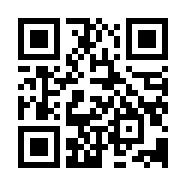
\includegraphics[width=8zw]{gazo/zenshotaishomei.png}
\end{wrapfigure}

熊野寮自治会は2019年から対処分戦略推進局(通称「処分局」)を設けて、毎週会議を行っています。処分局では被処分者と綿密に話し合いながら、上記処分を撤回させること、これ以上の学生処分をさせないという目的の下、処分問題についての広報活動や学内諸団体との連携を行っています。寮生だけでなく、寮外生も参加しています。(毎週火曜日20時から熊野寮食堂で会議してます)

また処分問題を全学的な問題として扱うために、熊野寮自治会処分局、法学部学生自治会処分対策小委員会、全学自治会同学会執行委員会(安田委員長)やその他有志によって全学処分対策委員会(全処対)が2020年3月に結成されました。全処対では上で述べたように恣意的な運用が可能な学生懲戒規程を撤廃し、これまで当局によって行われた処分を撤回するように求める署名を行っています。右記QRコードまたは\url{https://bit.ly/3ert3ta}から署名お願いします。

寮としてこうした積極的な行動をとるのは、無期停学処分の理由が寮自治会としての要求書提出行動や寮祭企画だったから、というだけではありません。\textbf{一人でも抑圧を受けている学生がいれば、それをみんなの問題として受け止めて行動することが学生自治会の役割だからです}。一人で処分の撤回を訴えても、当局は聞く耳を持たないでしょう。しかし、学生自治会として被処分者と一体となって動き、京大当局に圧力を掛けることができれば、当局は処分の撤回や軽減を考えざるを得なくなるでしょう。また、自治会として積極的に動くことは現在や未来の寮生、学生にとっても利益のあることです。先程も言ったように、この処分は京大の自由を奪おうとするものです。学生が声を上げる自由がなくなれば、当局が寮を廃止しようとしてきたり、学費を上げようとしてきた場合に、それに反対の声を上げ、学内外での運動を盛り上げることはできません。学内での学生の声を守るために、「不当な学生処分は絶対に許さない」という態度表明が必要です。


\subsection{12月集会}

\begin{wrapfigure}{r}{18zw}
    \vspace*{-\intextsep}
    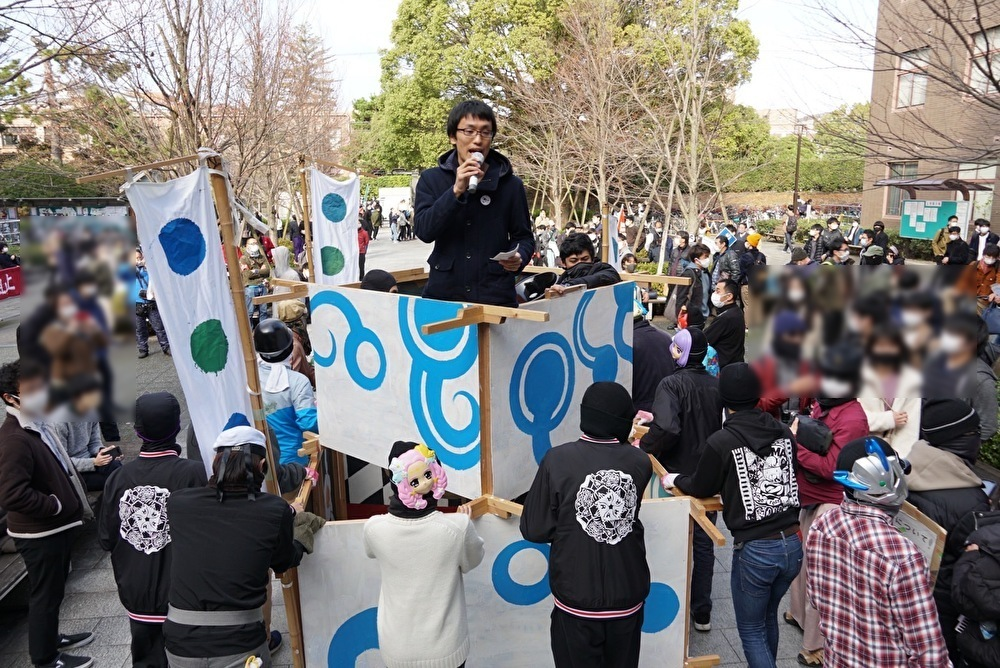
\includegraphics[width=18zw]{gazo/202112shukai.jpg}
    \captionsetup{labelformat=empty,labelsep=none}
    \caption{神輿に乗って演説する被処分者}
\end{wrapfigure}

全処対では時計台占拠処分に向けた呼び出しが来た当初から京大構内で集会を行って
きました。特に昨年12月9日には 2019、2020、2021年(前者2つは実行委員会主催)に
引き続いて、全処対主催で京大学生処分撤回・阻止12月緊急集会(通称「12月集会」)が行われました。この集会には熊野寮自治会を始めとして、文学部自治会学友会常任委員会などの学生自治会も賛同しました。当局は告示第9号を発し、集会開催を禁止し、集会に参加しないよう学生に呼びかけましたが、200 人規模の学生と教員と市民が大学構内の総人広場に集結し、無事やりきることができました。実際に処分を受けた学生や、処分問題に思うところがある教員や他大学の学生等から発言があり、広い陣形で集会を行うことができました。

この集会には2つの意義があると思います。まず、これだけ多くの学生が集えば、当局がいくら集会を禁止しようと集会できるのだと分かったことです。多くの学生が集えば表現の自由を守ることができるのです。逆に、表現の自由を守ろうという意志のもとにみんなが積極的に動かなければ、当局は簡単に学生の声を奪うことができたでしょう。自由は当局によって与えられるものではなく、それを守ろうという不断の努力で私たち学生が作るものです。もう1つは、当局に対して、処分撤回で一致する学生の力を見せつけることができたことです。2019年にも12月集会は同じ趣旨のもとで行われ、多くの学生を集めることで、一名の反省文なしの無期停学解除を勝ち取ることができました。多くの学生が集まれば集まるほど当局は無期停学の解除や学生処分の撤回をせざるをえない状況に追い込まれるはずです。


\subsection{お願い}
対処分戦略推進局はこれからも処分の撤回と処分阻止を目的に活動を進めていきます。これを読んでいらっしゃるみなさんも、京大当局の動きに注意深く目を向けてください。当局が何か変なことをしたら、諦めるのではなく、立ち上がってください。何をしたらいいのかわからなかったら、学部自治会や自治寮に顔を出してみてください。みなさんの力は京大の自由を守ることに絶対に繋がります。


\subsection{資料}

{\small
\begin{tcolorbox}[colback=white, colbacktitle=gray!30!white, coltitle=black, title=熊野寮生3名に対する無期停学処分の撤回を求める声明,breakable]

    \begin{flushright}
    京都大学熊野寮自治会
    \end{flushright}
    \begin{flushleft}
    京都大学総長 山極壽一 殿 
    \end{flushleft}
    
    2019年9月10日付けで熊野寮生3名に対し無期停学処分が下されました。3名の行った行為はどれも「職員の行為を妨害」したものであり、京都大学通則第32条第1項に規定する「学生の本分を守らない」行為であるとされたためです。今回の処分について、以下の2点から抗議します。
    
    \begin{enumerate}
        \item 大学職員の行為の正当性を検証する場がない\\
         3名の行為・言動は、京都大学当局(以下、当局)の一方的な決定とそれを遂行する職員に対する抗議として行われました。
    
         学生との話し合いが一切行われない中で、当局の決定に従う職員は自らの職務を強硬的・暴力的に全うしようとし、学生がそれに抗議すれば否応なしに処分が下されます。
        正当性が検証されていない職務行為への妨害を理由とした処分は撤回されるべきです。
        
        \item そもそも懲戒規程の内容が恣意的に運用できるものである\\
         「京都大学学生懲戒規程」(平成29年2月28日 達示第103号全部改正)において懲戒の対象は「学生の本分を守らない者」とされ、さらにここでは「京都大学の諸規程又は命令に違反した者」がその具体的な項目の一つとして記されています。
    
         これによって当局の意思決定及びそれに従う職員の行為に反する学生を恣意的に処分することができるため、この規程による処分は撤回されるべきです。
    \end{enumerate}
    
     今回の処分は、立て看板規制や吉田寮現棟明け渡し訴訟、11月祭への介入など、当局が学生への規制・弾圧を推進する渦中で行われています。
    
     今後も当局が抗議する学生を処分することは容易に想像でき、その影響は現在だけでなく未来の京大生にまで及びます。大学の在り方を考える学生の権利・主体性が剥奪され、当局の意思決定に学生が反論し抗議することすらできない状況は、理性と言論の府たる大学において看過されるものではありません。
    
     熊野寮自治会は、寮生3名に対する無期停学処分の即時撤回、今後同様の形で学生を処分しないこと、そして今後の大学運営においては当事者である学生との話し合いを踏まえたうえで意思決定がなされることを求めます。
    
    \begin{flushright}
    2019年10月18日
    \end{flushright}
    
    \vspace{5mm}
    \noindent ▼京都大学による公式発表「学生の懲戒処分について」(2019年9月12日)\\
    (\url{http://www.kyoto-u.ac.jp/ja/about/events_news/office/kyoiku-suishin-gakusei-shien/kosei/news/2019/190912_1.html})
    
    \begin{quotation}
    本学は、文学部4回生1名、工学部4回生1名、総合人間学部4回生1名を、令和元年9月10日付けで、以下のとおり懲戒処分とすることを決定しました。
    \begin{enumerate}
        \item 文学部4回生1名を、京都大学通則第32条に定める「学生の本分を守らない者」として、令和元年9月10日付けで同通則第33条に定める停学(無期)処分とした。
        \item 工学部4回生1名を、京都大学通則第32条に定める「学生の本分を守らない者」として、令和元年9月10日付けで同通則第33条に定める停学(無期)処分とした。
        \item 総合人間学部4回生1名を、京都大学通則第32条に定める「学生の本分を守らない者」として、令和元年9月10日付けで同通則第33条に定める停学(無期)処分とした。
    \end{enumerate}
    
    \vspace{4mm}
    \noindent 処分理由
    \begin{enumerate}
        \item 文学部学生
        
         当該学生は、平成30年8月9日、オープンキャンパス初日に本部構内のクスノキ東側に設置された巨大工作物の一部に座り込み、当該工作物を撤去しようとする職員の行為を妨害するなどした。
    
         また、当該学生は、平成30年9月27日及び同年10月18日、教育推進・学生支援部棟2階の厚生課窓口及び廊下において、不審者を取り押さえようとする職員の行為を妨害するなどした。
    
         これらのことは、京都大学学生懲戒規程第3条第5号「前各号に準ずる不適切な行為を行った」に該当し、京都大学通則第32条第1項に規定する「学生の本分を守らない」行為である。
    
         よって、本学は、今回の行為の事実関係について調査を行い、慎重に審議した結果、当該学生を停学(無期)処分とすることとした。
        
        \item 工学部学生
        
         当該学生は、平成30年9月27日及び同年10月18日、教育推進・学生支援部棟2階の厚生課窓口及び廊下において、不審者を取り押さえようとする職員の行為を妨害するなどした。
    
         また、当該学生は、平成30年10月3日、吉田南構内において立入禁止対象者を構外へ連れ出そうとする職員の行為を妨害するなどした。
    
         これらのことは、京都大学学生懲戒規程第3条第5号「前各号に準ずる不適切な行為を行った」に該当し、京都大学通則第32条第1項に規定する「学生の本分を守らない」行為である。
    
         よって、本学は、今回の行為の事実関係について調査を行い、慎重に審議した結果、当該学生を停学(無期)処分とすることとした。
        
        \item 総合人間学部学生
    
         当該学生は、平成30年9月27日及び同年10月18日、教育推進・学生支援部棟2階の厚生課窓口及び廊下において、不審者を取り押さえようとする職員の行為を妨害するなどした。
    
         このことは、京都大学学生懲戒規程第3条第5号「前各号に準ずる不適切な行為を行った」に該当し、京都大学通則第32条第1項に規定する「学生の本分を守らない」行為である。
    
         よって、本学は、今回の行為の事実関係について調査を行い、慎重に審議した結果、当該学生を停学(無期)処分とすることとした。
        
    
    \end{enumerate}
    \end{quotation}
    
    \vspace{5mm}
    \noindent ▼今回の処分で用いられた規程\\
    「京都大学学生懲戒規程」(平成29年2月28日 達示第103号全部改正)
    \url{http://www.kyoto-u.ac.jp/ja/about/organization/other/revision/documents/h28/t103-28.pdf}
    
    \vspace{5mm}
    \noindent ▼補足\UTF{2160}.不審者取り押さえ時の状況
    
     3名に共通する処分理由である上記の「平成30年9月27日及び同年10月18日」の件は、熊野寮自治会による要求書提出の際に起こった出来事です。この際、2017年7月25日付で京都大学を放学処分となり、同年10月2日付で学外者として敷地内立入禁止とされた\UTF{9AD9}田暁典がストッキングとフルフェイスヘルメットを被り、水色のネズミの着ぐるみを装って提出行動に参加していました。10月18日の要求書提出後、職員約8名が彼を取り押さえ、顔を隠した素性不明の不審者として警察に引き渡し、不退去罪の現行犯として逮捕させました。
    
     職員は退去しようとしていた\UTF{9AD9}田を大人数で取り押さえ、その手を踏みつけて流血させ、彼の退去を暴力的に阻止していました。この取り押さえ方に対し、寮生3名は職員と高田の間に割って入る、職員を高田から引き剥がすなどして、それを阻止しようとしました。
    
    \vspace{5mm}
    \noindent ▼補足\UTF{2161}.近年の京大内の管理強化について
    
     ここ数年、大学職員は顔を隠して活動する学生を取り締まっています。顔を隠した状態で学内に入ろうとする学生に対し素顔をさらせと職員が要求し、拒否した学生に対しては不審者と断定し学外に強制的に排除します。顔を確認することで個人を特定し、学内での行動を逐一監視したり、学部・研究室の教授を通しての脅しをかけたりなど、あらゆる形で学生に対し圧力をかけています。オープンキャンパスなどで着ぐるみを着て学内で宣伝活動している学生もいますが、顔を隠している学生は無条件で全員排除というわけではなく、職員の一存で強制排除されるかどうかが決まります。
\end{tcolorbox}


\begin{tcolorbox}[colback=white, colbacktitle=gray!30!white, coltitle=black, title=2019年学部入試における「オルガ像」設置を理由とした学生処分についての抗議文,breakable]

    \begin{flushleft}
    京都大学総長 山極壽一殿  京都大学理学部長 平島崇男殿
    \end{flushleft}
    
     2020年1月28日付けで、本学理学部に所属する学生1名に対して譴責処分が下されました。2019年度前期学部入試において、学内にアニメキャラクターを模した像(いわゆる「オルガ像」)を設置したこと、入試当日の職員に対する言動、職員の指示に対し即座に従わなかったことが主な処分理由とされています。
    
     熊野寮自治会はこの処分に対して以下2点の理由から強く抗議します。
    \begin{enumerate}
        \item 当該学生の行動はなんら問題ではない
    
         今回の処分理由において、当該学生の言動(「オルガ像」の設置や職員とのやり取り)が入試業務を妨害したとされています。しかしながら、当時の入試対策委員長だった酒井敏教授によると
        \begin{itemize}
            \item 入試当日、試験監督の間ではオルガ像の設置や
            当該学生の言動は全く問題になっていなかったこと
            \item むしろ職員の過剰な対応
            (試験時間中の工作物の撤去や当該学生に対する言動)
            が問題になったこと
        \end{itemize}
        が分かっています\footnote{自由を謳う京大が「不自由」になっている...学生が語るその現実、現代ビジネス\\
        \url{https://gendai.ismedia.jp/articles/-/70539}}\footnote{自由の学風/京大変人講座,Twitter\\
        \url{https://twitter.com/orita_hikoichi/status/1181451625442865153}}。
        
         この事実からも「オルガ像」の設置は入試業務の進行に対して何ら実害を与えていないものであることは明らかです。
        \item 処分規定の恣意的な運用である
    
         これまで当局は学部入試における工作物の設置を京大の文化として好意的に取り上げてきました。しかしながら、入試担当者すら問題にしなかった当該学生の言動を、さも深刻な妨害があったかのように取り上げ処分を行うことは明らかに処分規程の恣意的な運用です。
    
         この間、入試に限らず、当局は学生の自主的活動を一方的に「迷惑行為」「学生の本分に反する」として規制してきました。このように問題でないことを問題として取り上げる形での学内規則の恣意的な運用が今後も懸念されます。
    \end{enumerate}
    
    
     熊野寮自治会は2019年10月18日付けの声明文で、恣意的に運用できる規程を用いた処分を二度と行わないこと、大学の運営に際しては学生との話し合いを踏まえた意思決定をすることなどを求めましたが、その要求が無視され再び一方的な処分が繰り返されています。熊野寮自治会としてこの事態を看過することはできません。当事者である学生を抜きに
    した意思決定、および恣意的な処分を用いた学生への威圧行為を取りやめることを求めるとともに、今回の譴責処分に対し強く抗議します。
    
    \begin{flushright}
    2020年7月17日  京都大学熊野寮自治会
    \end{flushright}
    
\end{tcolorbox}

\begin{tcolorbox}[colback=white, colbacktitle=gray!30!white, coltitle=black, title=公開要求書(2021年11月26日)の要求3,breakable]
    3.現在進められている処分手続きを撤回すること
    
    昨年行われた時計台占拠に参加したとして、村中副学長が委員長である研究科長特別委員会より8名(当初は9名)が呼び出しがなされ、処分手続きが進められている。当該は証拠の事前開示、聴き取り調査に関して弁護士含む同伴者の同席、公開されることがなければ調査に際して当該の学生が威圧されることを防ぎ、その心理的安全を担保することはできず、そうでなければ調査及び弁明の場として公正なものではなく、応じることはできないとしてきた。上記の要求を「教学的指導の観点」を口実に特別委員会は拒否している。現在処分手続きが進められ、「処分の言い渡し」として当該らに呼び出しがかかっているが、このような状況下で進められる処分手続きは正当なものとして認められない。また、時計台占拠の正当性について一切寮自治会と交渉することなく、参加したとされる学生を一方的に処分することは学生自治の侵害であり、学問の自由の侵害である。ただちに現在進められている処分手続きを撤回すべきである。
\end{tcolorbox}

}